% Source of figures/pipeline.pdf (Fig. 1). Compile with pdflatex to regenerate.
\documentclass[border=3pt]{standalone}
\usepackage[T1]{fontenc}
\usepackage{lmodern}
\usepackage{amssymb}
\usepackage{tikz}
\usetikzlibrary{arrows.meta,backgrounds,fit}
\definecolor{pass}{HTML}{1B7F4B}
\definecolor{fail}{HTML}{B3261E}
\definecolor{held}{HTML}{9A6700}
\definecolor{rt}{HTML}{2A78D6}
\definecolor{ev}{HTML}{EB6834}
\newcommand{\ok}[1]{{\color{pass}$\checkmark$\,#1}}
\newcommand{\no}[1]{{\color{fail}$\times$\,#1}}
\newcommand{\hd}[1]{{\color{held}$\sim$\,#1}}
\definecolor{gate}{HTML}{1F4E8C}
\newcommand{\gd}[1]{{\color{gate}$\bullet$\,#1}}
\begin{document}
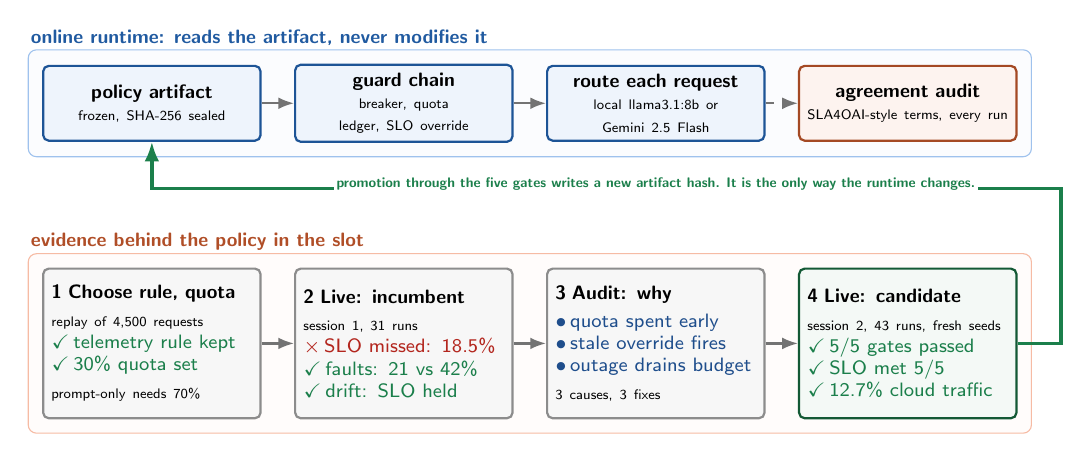
\begin{tikzpicture}[
  font=\sffamily\scriptsize,
  rbox/.style={draw=rt!70!black, fill=rt!8, rounded corners=2pt, thick, align=center,
               inner sep=3pt, text width=2.55cm, minimum height=0.95cm},
  ebox/.style={draw=black!45, fill=black!3, rounded corners=2pt, thick, align=left,
               inner sep=3pt, text width=2.55cm, minimum height=1.9cm},
  a/.style={-{Latex[length=2mm]}, thick, black!55},
]
% ---------------- runtime lane (y = 0)
\node[rbox] (art)   at (0.0,0) {\textbf{policy artifact}\\{\tiny frozen, SHA-256 sealed}};
\node[rbox] (guard) at (3.2,0) {\textbf{guard chain}\\{\tiny breaker, quota ledger, SLO override}};
\node[rbox] (route) at (6.4,0) {\textbf{route each request}\\{\tiny local llama3.1:8b or Gemini 2.5 Flash}};
\node[rbox, draw=ev!70!black, fill=ev!8] (agr) at (9.6,0) {\textbf{agreement audit}\\{\tiny SLA4OAI-style terms, every run}};
\draw[a] (art) -- (guard);
\draw[a] (guard) -- (route);
\draw[a, dashed] (route) -- (agr);
\begin{scope}[on background layer]
  \node[draw=rt!45, fill=rt!2, rounded corners=3pt, inner sep=5pt, fit=(art)(guard)(route)(agr)] (rtbox) {};
\end{scope}
\node[anchor=south west, font=\sffamily\scriptsize\bfseries, text=rt!75!black, inner sep=1pt]
  at (rtbox.north west) {online runtime: reads the artifact, never modifies it};

% ---------------- evidence lane
\node[ebox] (g1) at (0.0,-3.05) {\textbf{1\;Choose rule, quota}\\[2pt]
  {\tiny replay of 4,500 requests}\\ \ok{telemetry rule kept}\\ \ok{30\% quota set}\\[2pt]
  {\tiny prompt-only needs 70\%}};
\node[ebox] (g2) at (3.2,-3.05) {\textbf{2\;Live: incumbent}\\[2pt]
  {\tiny session 1, 31 runs}\\ \no{SLO missed: 18.5\%}\\ \ok{faults: 21 vs 42\%}\\ \ok{drift: SLO held}};
\node[ebox] (g3) at (6.4,-3.05) {\textbf{3\;Audit: why}\\[2pt]
  \gd{quota spent early}\\ \gd{stale override fires}\\ \gd{outage drains budget}\\[2pt]
  {\tiny 3 causes, 3 fixes}};
\node[ebox, draw=pass!70!black, fill=pass!5] (g4) at (9.6,-3.05) {\textbf{4\;Live: candidate}\\[2pt]
  {\tiny session 2, 43 runs, fresh seeds}\\ \ok{5/5 gates passed}\\ \ok{SLO met 5/5}\\ \ok{12.7\% cloud traffic}};
\draw[a] (g1) -- (g2);
\draw[a] (g2) -- (g3);
\draw[a] (g3) -- (g4);
\begin{scope}[on background layer]
  \node[draw=ev!45, fill=ev!2, rounded corners=3pt, inner sep=5pt, fit=(g1)(g2)(g3)(g4)] (evbox) {};
\end{scope}
\node[anchor=south west, font=\sffamily\scriptsize\bfseries, text=ev!75!black, inner sep=1pt]
  at (evbox.north west) {evidence behind the policy in the slot};

% ---------------- promotion arrow: session 2 -> artifact
\draw[-{Latex[length=2.5mm]}, very thick, pass]
  (g4.east) -- ++(0.55,0) |- ([yshift=-4mm]rtbox.south) -| (art.south);
\node[font=\sffamily\tiny\bfseries, text=pass, fill=white, inner sep=1pt] at (6.4,-1.02)
  {promotion through the five gates writes a new artifact hash. It is the only way the runtime changes.};
\end{tikzpicture}
\end{document}
